\section{Tightly Integrated Building Information System Architecture}

The first building information systems became commercially available in the 1970's ~\cite{gardner1987energy}.  
Historically, building management 
systems were constructed as a collection of control loops, which progressed from pneumatic to analog to digital.
These control loops largely form the foundation for the design decisions made in building information systems.  
This section gives a quick overview of the architecture, bottom-up and describes how each stage is built around
the concept of loops and supervisory control.  We then describe some of the short-comings of this architecture
and give an overview of how we address it in a system called StreamFS -- described in more details in
the remaining chapters.

\begin{figure}[t!] %htbp
\centering
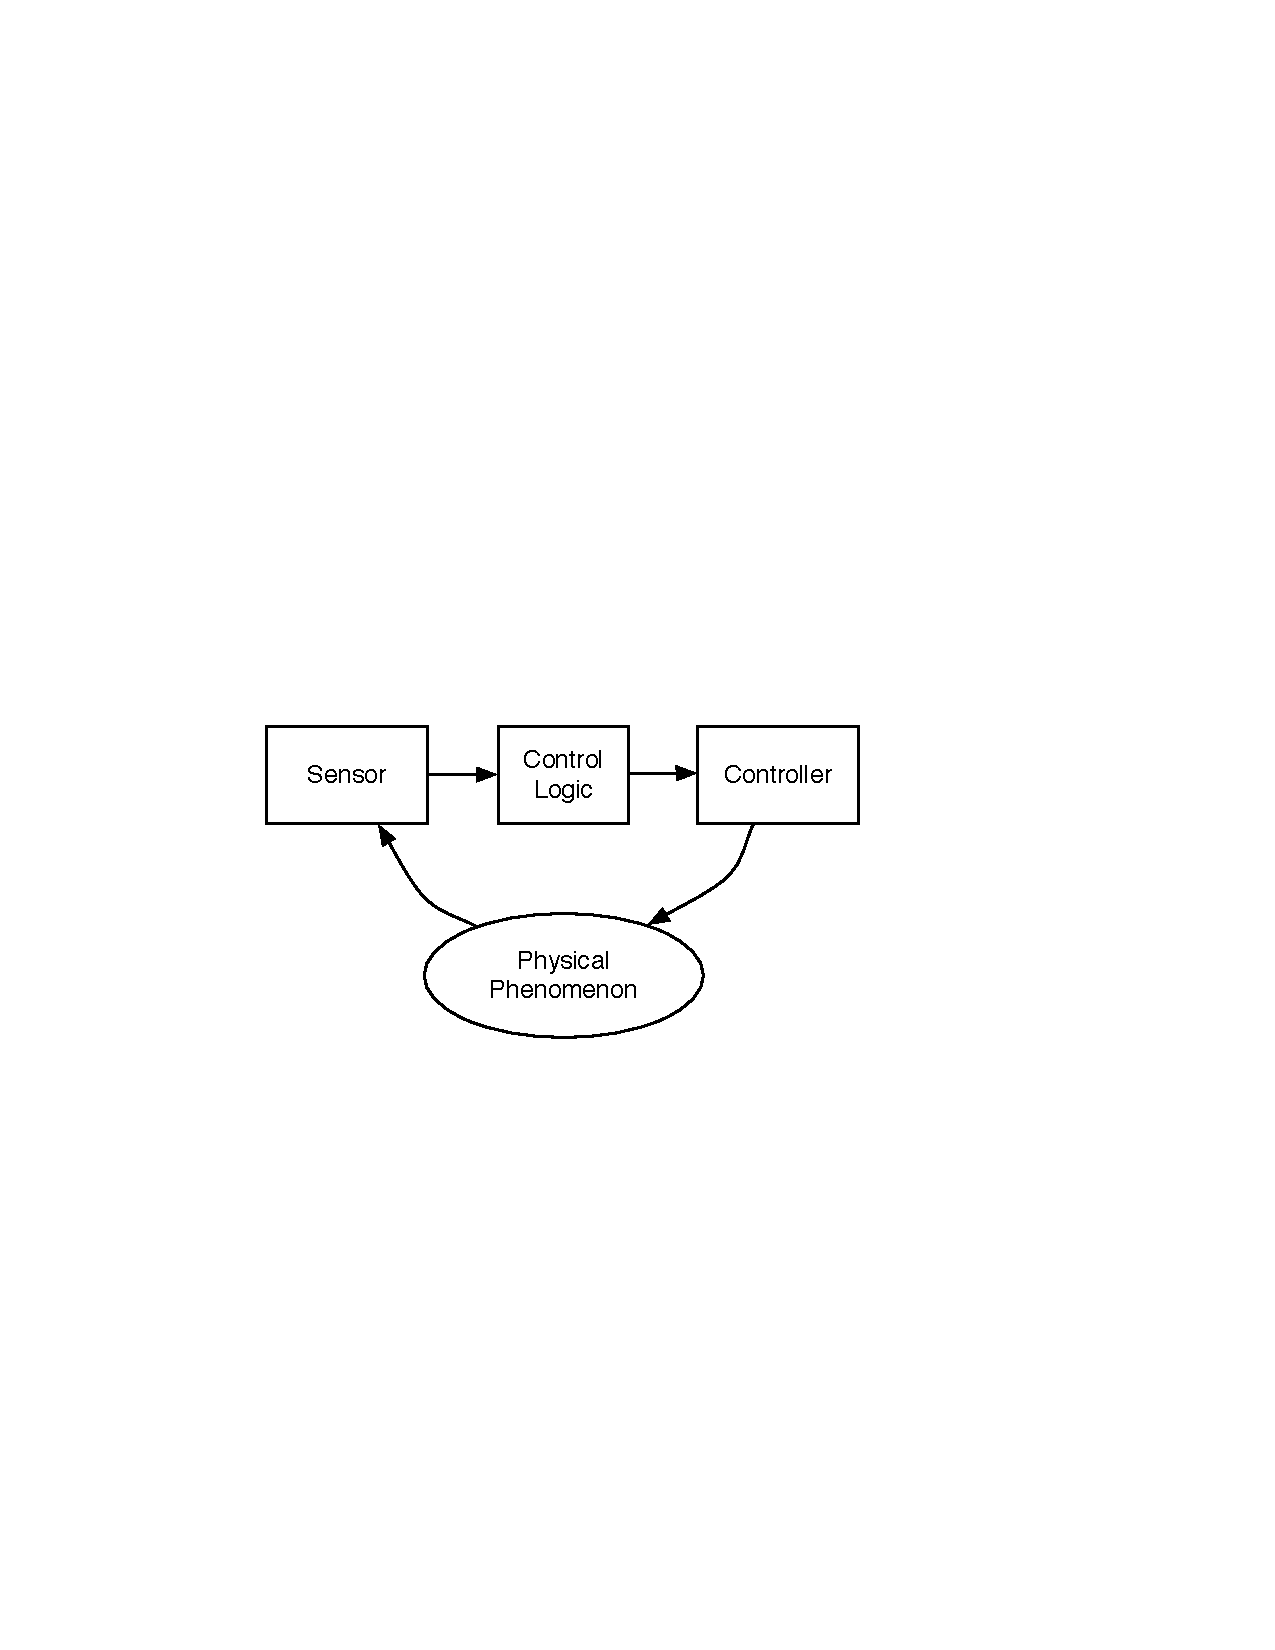
\includegraphics[width=0.50\columnwidth]{figs/control_loop}
\caption{General building control loop.}
\label{fig:control_loop}
\end{figure}

\subsection{Control Loops and The Outstation}
\label{sec:control_loops}
Each loop is defined by a control domain consisting of a sensor, an actuator, and a control mechanism.  The control mechanism
become logic based when signals from sensors moved to the digital domain.  However, the basic control principle is based
entirely on local control loops, with the implicit assumption that these loops are independent.
Figure~\ref{fig:control_loop} shows a high-level control loop.  A simple control loop in the building is one that controls
the temperature in a space.  It has a temperature sensor as the input and uses the temperature set-point parameter to 
decide when and which actuators to activate.
For temperature control, this actuation controls the vent that lets cool air into the space.  This causes the temperature
to fall until a lower-bound is reached and the control logic re-activates the fans and heating/cooling system.

The figure also shows the basic structure inside an outstation.  An outstation is a box that contains up to several control boards, each
wired to one or more sensors and one or more actuators.  The outstation is typically close to the sensors and actuators (in the same room)
and contains all the control logic for the local plant.  Inside the control logic there is a CPU and some memory.  The memory
contains the control program and some space for sensor readings.  It is directly wired to the sensors and actuators through
a series of buses and shown in Figure~\ref{fig:control_box}.

\begin{figure}[t!] %htbp
\centering
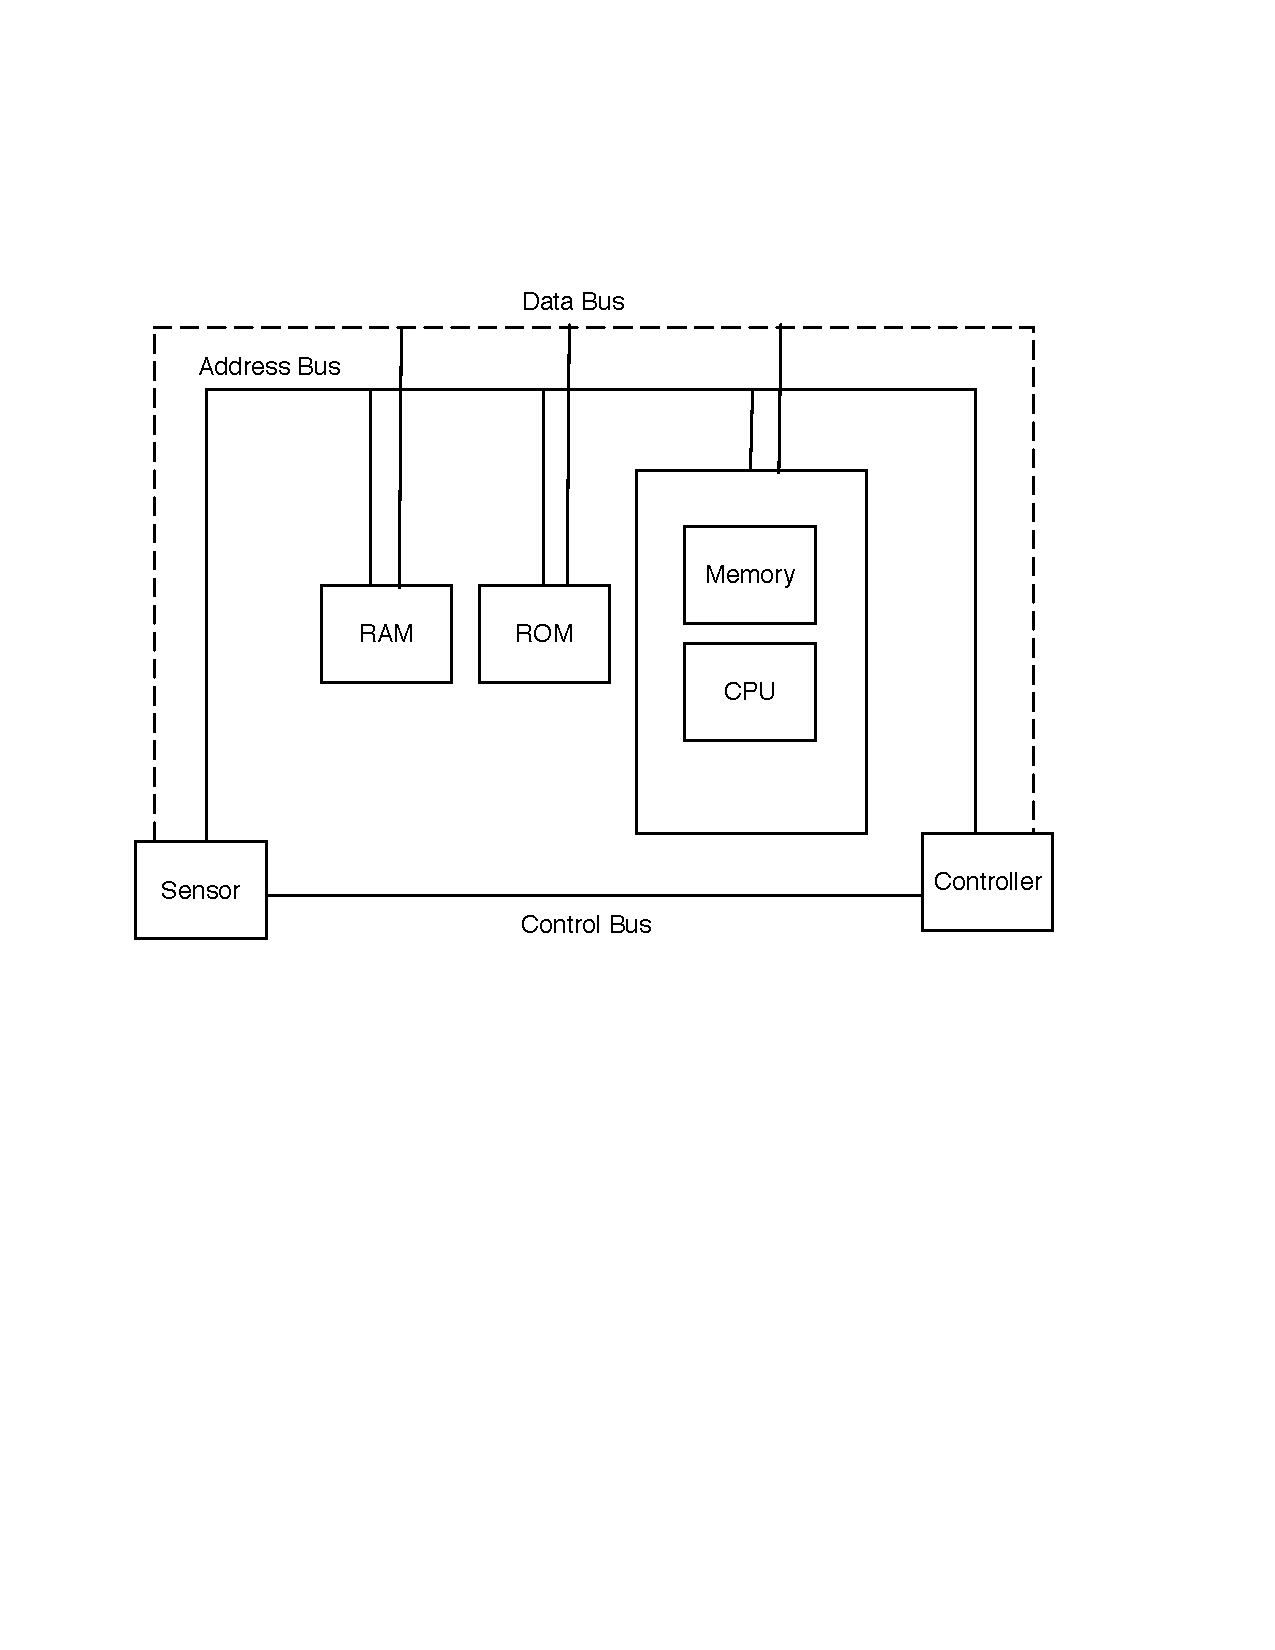
\includegraphics[width=0.50\columnwidth]{figs/control_box}
\caption{High-level control board architecture.}
\label{fig:control_box}
\end{figure}

As readings from the sensors are taken, they are placed in RAM.  The amount of RAM is limited and can get filled up, so it is important
to schedule periodic collection tasks from the central station -- the building management system (BMS).  The control logic is typically
written in ROM and can only be changed by the equipment or BMS vendor.  The input parameters are set at the BMS and they dictate the operational dynamics
of the control scheme in reaction to the input~\cite{BMS_book}.
Outstations are distributed through the building and are essentially running independent of one another.  In order to enable centralized 
monitoring and control, they are networked together and report some of the sensor readings and control-logic state to a central outstation.

\subsection{Central Outstation and Communication Protocols}
The central outstation is typically a Microsoft Windows-based PC connected to the outstation through either RS-485/modbus or Ethernet.
The user interacts with the system through a graphical interface, constructed from the schematics for the building or the schematics
for the component in the system that is being monitored.  The BMS running on the PC communicates with outstations through either a 
vendor-specific, proprietary protocol or an open one like BACNet~\cite{Bacnet} or LonTalk~\cite{LonTalk}.  Note, 
we focus on BACNet, but the similar features exist in other protocols, such as LonTalk.  

\begin{figure}[h!] %htbp
\centering
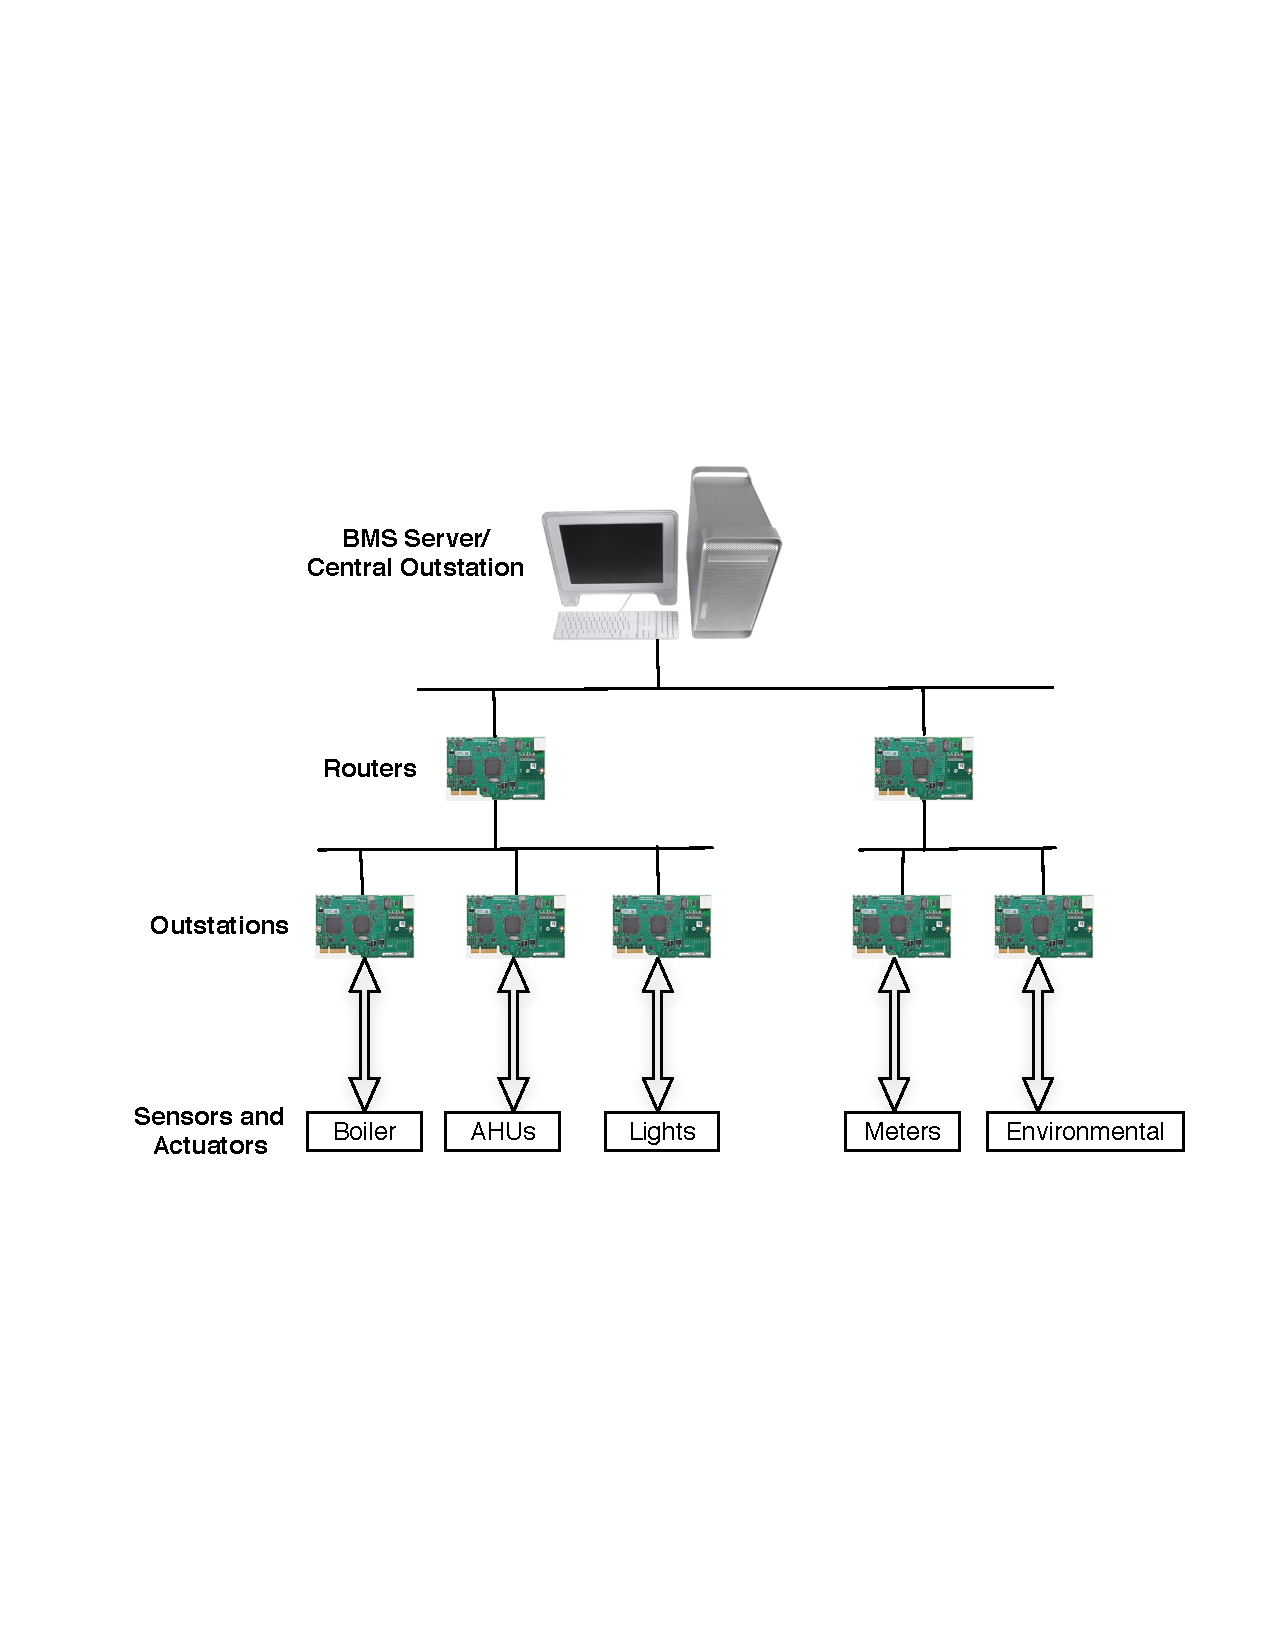
\includegraphics[width=0.50\columnwidth]{figs/BMS_network}
\caption{BMS network architecture.}
\label{fig:bms_network}
\end{figure}

Both protocols define both a wire protocol and packet structure for communicating with outstations and each other.  They also define a high-level
naming scheme for sensors in the building, called `points'.  A point can also refer to a non-physical object, like a schedule of operation.
It is common for both lights and temperature sensors to run on a daily, weekly, and seasonal schedules.  Such schedule are captured
by the \emph{schedule object} in BACNet.  
% BACNet also exposes devices as a collection of different object types.  
Each object contains a set of properties that can 
be read and/or written.  A device is identifiable through a name or address on the network, each object has a unique identifier and is one of
many types.  Examples of object types includes the following: input, output, value, analog~\cite{Bacnet}.  

These protocols also provide a mechanism for discovery .  Each [device, object name/id, property name/id] tuple forms a name.
This name is exposed by the protocol-server to the application.  All the names are set by the vendor and the are shown through the graphical interface
of the BMS.  
% constructed from the building schematics, is also designed and constructed by the vendor.  
The building manger is the primary user of the BMS,
so rather than expose the underlying protocol, he/she interacts with the building via the graphical interface.

In order to interact with the underlying sensor and actuator layer, the application must use a stub that communicates directly with the 
sensor/actuator through the BACnet stack.  External communication stubs are recognized similarly to sensors/actuators.  They are represented 
as a collection of 
objects with readable/writable properties.  An example service that is provided in BACNet is  \texttt{WhoIs} and \texttt{EventNotification}.
The former is a broadcast service that is used for discovery of other objects, the latter is used for setting alarms on the sensor data that
are reported by the BACNet enabled devices on the network in the outstation layer.  There are many other types of events that are supported 
and over 50 types of object types in the baseline protocol, which is extensible.  Device and object names that are added have no restriction
on either the number of characters (specified by the vendor) or the encoding.


\begin{figure}[t!] %htbp
\centering
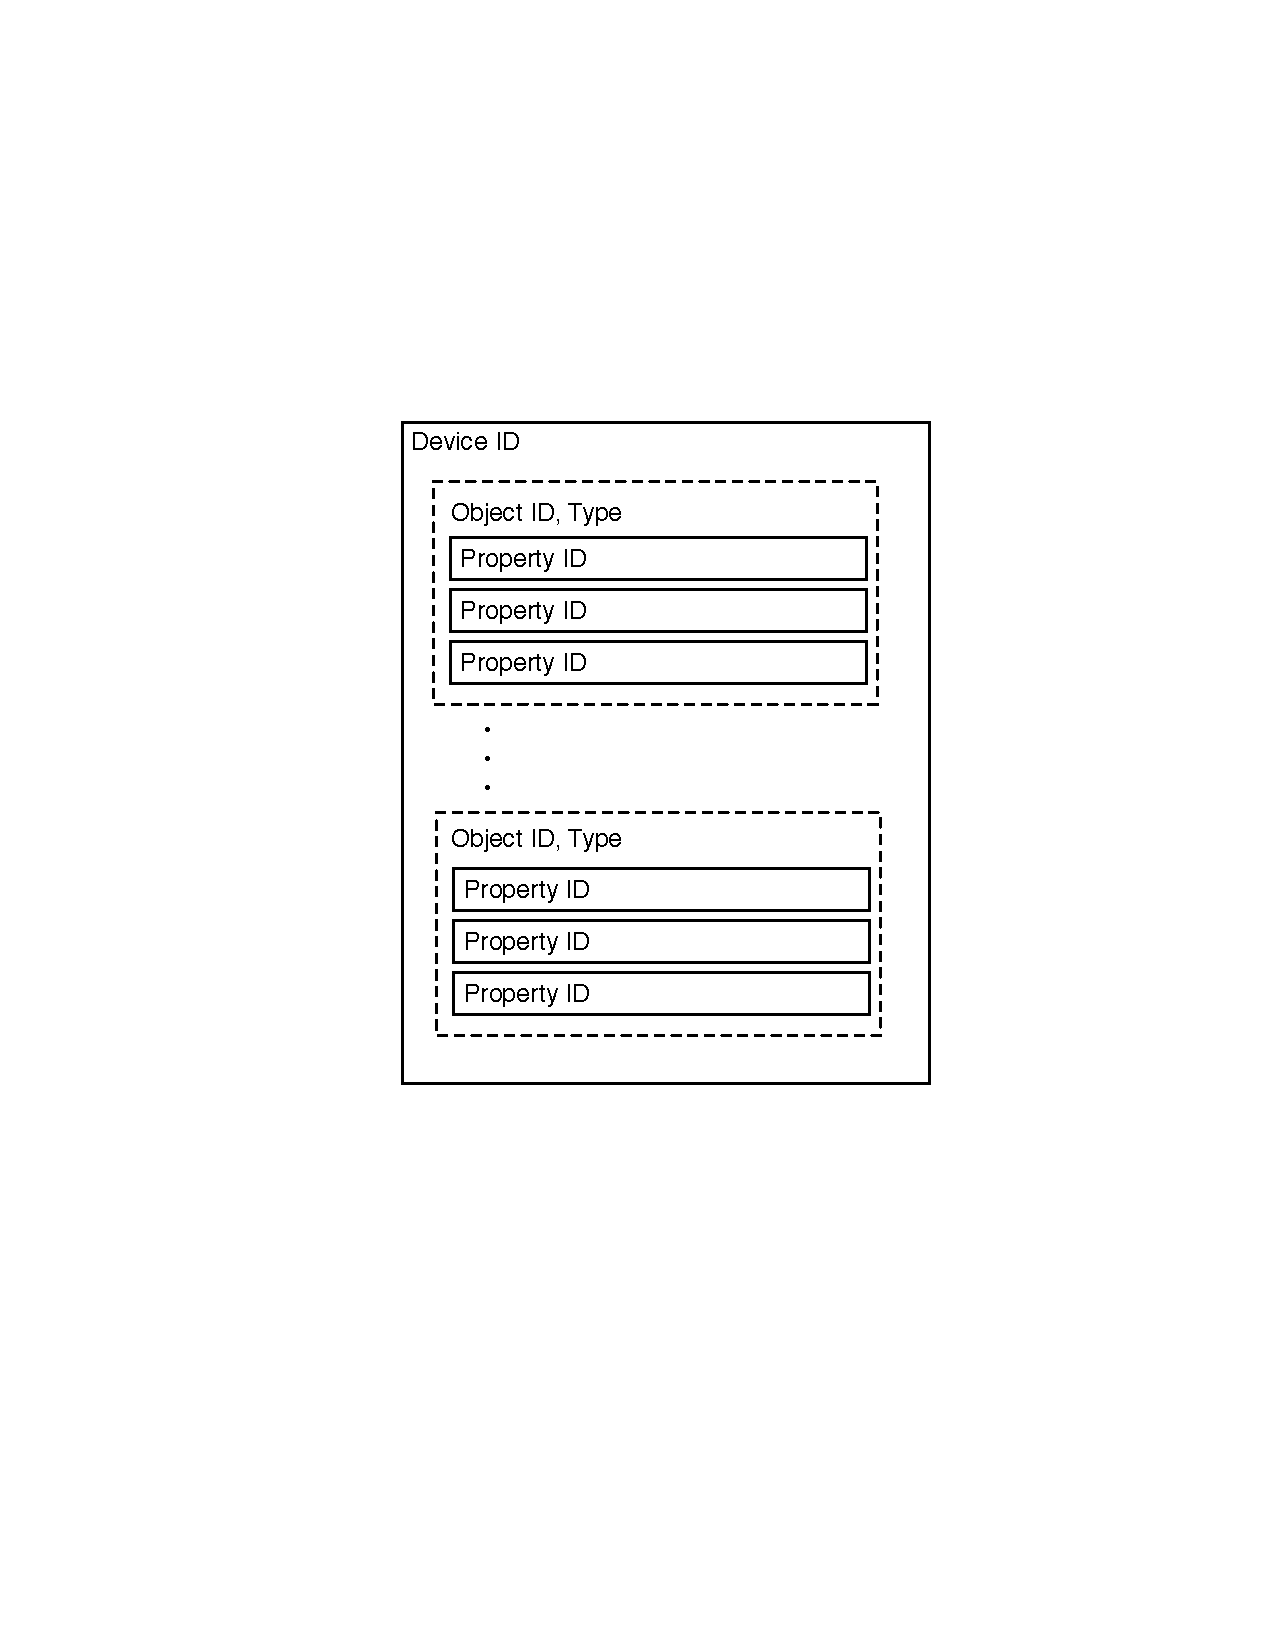
\includegraphics[width=0.25\columnwidth]{figs/bacnet_device}
\caption{BACNet device example.}
\label{fig:bacnet_device}
\end{figure}